\documentclass[../../dd.tex]{subfiles}

\begin{document}

	\chapter{User Interface Design}

	We have already describe all the main interfaces that the application can show on the chapter 3.1.1 of the RASD. On that chapter we have already describe also the input and the action that each user can do, and show a possible graphic layout of the pages using some mock object. On this chapter we focus on the navigation between this pages and we describe in a more specific way the input form. To do that we use a UX diagram UML. With this diagram we give a global overview of all the possible pages with the relative forms. 
	
	\begin{figure}[H]
				\centering
				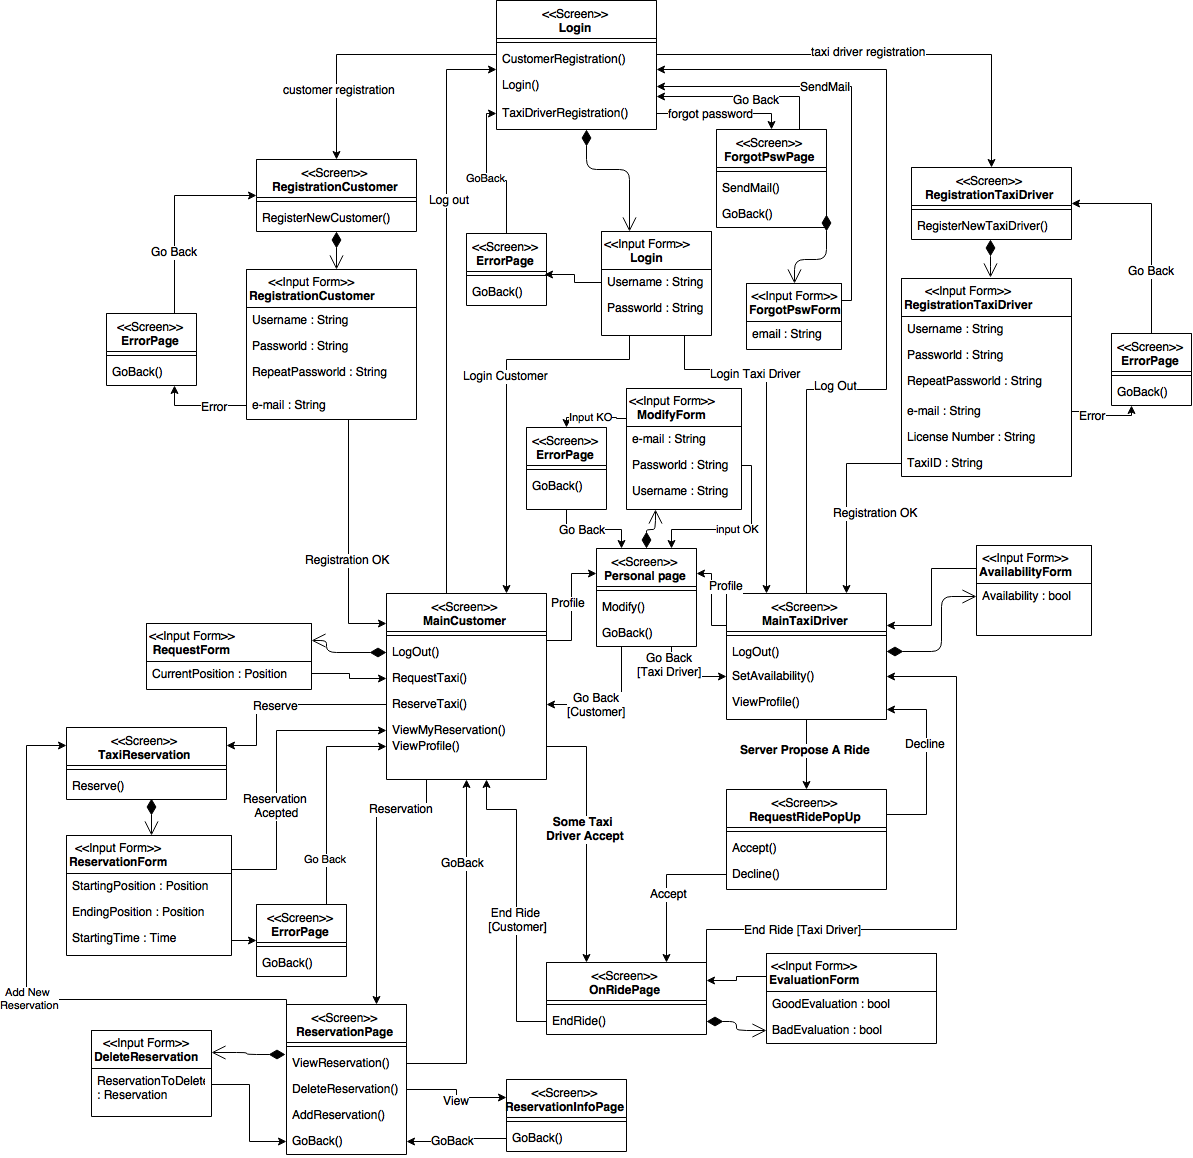
\includegraphics[width=\textwidth, scale=0.5]{../images/UserInterfaces.png}
			\caption{UX Diagram UML}\label{fig:UXDiagram}
		\end{figure}
		
Note: We use [Customer] or [TaxiDriver] on the transition to identify the return page if you are respectively logged as a customer or a taxi driver. We do this because the incoming pages have no differences if you are logged as a customer or as a taxi drivers.
Note: The transition with the bold text is transition that not depends on the input of the user. So, this kind of translations are, for example, pop up that is showed when on the system something is happen. E. g. a taxi driver that is on his main page can pass on the RequestRidePopUp screen without make any move, simply the pop up is showed when the system ask to the taxi driver if he want to take that ride.

\end{document}